% Petteri is responsible for this section
\section{Minimum, Maximum, and Mean Distances}
Present the plots of minimum, maximum and mean distances for each \( L_p \) and discuss the results. How the curves are behaving when \( k \) increases? Can you characterize the form of curves? What is the effect of \( p \)? If a curve seems to be converging, tell also the value that it is approaching.
\subsection{Min-Max-Mean Distance}

P values lower than 1 grow polynomamially.
The following equation shows the proportionality.


\begin{equation}
    \forall p < 1, \lim_{k \to \infty} \left( \sum_{i=1}^{k} |x_i|^p \right)^{\frac{1}{p}} \propto k^{\frac{1}{p}}
\end{equation}


and p value 1 grows linearly.
\begin{equation}
    \forall p = 1, \lim_{k \to \infty} \left( \sum_{i=1}^{k} |x_i|^p \right)^{\frac{1}{p}} \propto k
\end{equation}

P values greater than 1 grow as p roots of k. The reasoning comes from the norm equation:

\begin{equation}
    \forall p > 1, \lim_{k \to \infty} \left( \sum_{i=1}^{k} |x_i|^p \right)^{\frac{1}{p}} \propto \sqrt[p]{k}
\end{equation}


For all the curves, they can be formulated as curves according to their growth rate, polynomial, linear, or p-root. For the \(\infty\)-norm, the curve can be formulated as a multiplicative inverse curve approaching 1 as \(k\) approaches infinity. The shape of that curve is shown in the figure \ref{fig:meanmax_lp_infty}. The rest of the curves for all other norms can be found from the codefile from the appendix.

\begin{equation}
    \lim_{k \to \infty} \max_{i=1,\ldots,k} |x_i| = 1
\end{equation}

\FloatBarrier  % Ensures figure stays close to this text

\begin{figure}[htbp]
    \centering
    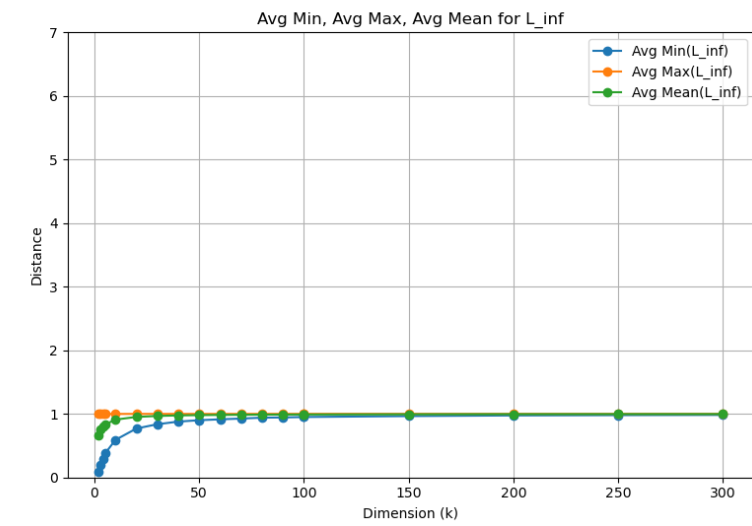
\includegraphics[width=0.9\linewidth,height=0.35\textheight]{meanmax_lp_infty.png}
    \caption{\emph{Mean-Max-Mean} for $L_{\infty}$}
    \label{fig:meanmax_lp_infty}
\end{figure}

All the norms except for \( L_\infty \) diverge as \(k\) increases. However, the \( L_\infty \) converges to one. Mathematically, this follows from the equation for the \( L_\infty \) norm. The values generated are between 0 and 1, and thus the maximum value will be one as \(k\) approaches infinity.

\FloatBarrier  % This makes sure the following text and figure stay close.
